% =====================================================================
%  Fig. 1 (clean redraw) -- end-to-end pipeline of the study, standalone TikZ.
%
%  Build : tectonic fig_pipeline_clean.tex   (XeTeX; page = 17.8 cm wide x 8.97 cm high)
%  Style : MLOps-architecture look (Kreuzberger et al.): light-grey stage panels with a
%          blue letter tag, white boxes with thin dark borders, one thin strip of secondary
%          text per panel, dashed grey zone separators, one legend row.
%  Colours (only these): panel E7E7E7, strip F4F4F4, box white / 404040 (0.5 pt), accent blue 4472C4,
%          "ours" fill DCE6F5 / blue 0.9 pt, text 222222, separators + zone names A6A6A6, arrows 404040.
%  Type  : Helvetica; panel titles bold 8 bp, box text 7.5 bp, strips/legend/labels 7 bp (nothing below
%          7 bp).  Sizes are given in TeX pt = bp x 1.00375 (8.03 / 7.53 / 7.03).
%  Layout: top zone = panels A, B; bottom zone = panels C, D (all coordinates in cm, origin bottom-left;
%          the bounding box is fixed by \useasboundingbox so the page is exactly 17.8 cm wide).
%  Flow  : A -> B along the top; one return line from B4 to the input column of C; C -> D below.
%          Solid arrows = data flow, dashed arrows = label flow.
% =====================================================================
\documentclass[tikz,border=2pt]{standalone}
\usepackage{fix-cm}
\usepackage[T1]{fontenc}
\usepackage[scaled=1]{helvet}
\renewcommand\familydefault\sfdefault
\usepackage{fontawesome5}
\usetikzlibrary{arrows.meta}
% ---- type sizes (TeX pt; 8.03 pt = 8 bp, 7.53 pt = 7.5 bp, 7.03 pt = 7 bp) ----
\newcommand{\fTitle}{\fontsize{8.03}{9.4}\selectfont\bfseries}   % panel titles
\newcommand{\fLetter}{\fontsize{8.03}{9.4}\selectfont\bfseries}  % panel tag letter
\newcommand{\fBox}{\fontsize{7.53}{8.6}\selectfont}              % box text
\newcommand{\fZone}{\fontsize{7.53}{8.6}\selectfont\bfseries}    % zone names
\newcommand{\fSmall}{\fontsize{7.03}{8.2}\selectfont}            % strips, legend, edge labels
\newcommand{\fRQ}{\fontsize{7.03}{8.2}\selectfont\bfseries}      % RQ tags
\newcommand{\fSmallI}{\fontsize{7.03}{8.2}\selectfont\itshape}      % strips and arrow labels (italic)
\DeclareMathSizes{8.03}{8.03}{7.03}{7.03}
\DeclareMathSizes{7.53}{8.03}{7.03}{7.03}
\DeclareMathSizes{7.03}{8.03}{7.03}{7.03}
% ---- palette ----
\definecolor{panelF}{HTML}{E7E7E7}\definecolor{stripF}{HTML}{F4F4F4}
\definecolor{blueC}{HTML}{4472C4}\definecolor{oursF}{HTML}{DCE6F5}
\definecolor{txtC}{HTML}{222222}\definecolor{zoneC}{HTML}{A6A6A6}
\definecolor{ink}{HTML}{404040}
\definecolor{detC}{HTML}{555555}\definecolor{greyT}{HTML}{595959}\definecolor{greyD}{HTML}{7F7F7F}  % detail lines, strips/labels/adapted titles, adapted details
\definecolor{oursT}{HTML}{2F5597}\definecolor{verC}{HTML}{D55E00}                                      % emphasis: dark blue, vermilion
\newcommand{\md}{\ \textperiodcentered\ }
\newcommand{\bT}[2]{{\bfseries\color{#1}#2}}                                       % box title: bold, 7.5 bp (node font), colour #1
\newcommand{\bD}[2]{{\fontsize{7.03}{8.2}\selectfont\color{#1}#2}}                 % box detail line: regular 7 bp, colour #1
\newcommand{\cylry}{0.062}
\tikzset{
  >=Stealth,
  every node/.style={text=txtC, inner sep=0pt, outer sep=0pt, font=\fBox},
  panel/.style={fill=panelF, draw=none, rounded corners=2.5pt},
  box/.style={draw=ink, fill=white, line width=0.5pt},
  ours/.style={draw=blueC, fill=oursF, line width=0.9pt},
  edge/.style={draw=ink, line width=0.6pt, -{Stealth[length=3.6pt,width=3.0pt]}},
  dedge/.style={edge, dash pattern=on 2.2pt off 1.6pt},
  lineplain/.style={draw=ink, line width=0.6pt},
  dlineplain/.style={draw=ink, line width=0.6pt, dash pattern=on 2.2pt off 1.6pt},
  sep/.style={draw=zoneC, line width=0.5pt, dash pattern=on 3pt off 2.2pt},
  axis/.style={draw=ink, line width=0.5pt, -{Stealth[length=3.6pt,width=3.0pt]}},
  tick/.style={draw=ink, line width=0.5pt},
}
% data store: cylinder with flat caps; #1 style, #2 #3 lower-left, #4 #5 upper-right
\newcommand{\cyl}[5]{%
  \pgfmathsetmacro{\cylrx}{(#4-#2)/2}\pgfmathsetmacro{\cyltop}{#5-\cylry}\pgfmathsetmacro{\cylbot}{#3+\cylry}%
  \draw[#1] (#2,\cyltop) -- (#2,\cylbot) arc[start angle=180,end angle=360,x radius=\cylrx cm,y radius=\cylry cm]
    -- (#4,\cyltop) arc[start angle=0,end angle=180,x radius=\cylrx cm,y radius=\cylry cm] -- cycle;
  \draw[#1,fill=none] (#2,\cyltop) arc[start angle=180,end angle=360,x radius=\cylrx cm,y radius=\cylry cm];}
\newcommand{\cylsmall}[5]{%
  \pgfmathsetmacro{\cylrx}{(#4-#2)/2}\pgfmathsetmacro{\cyltop}{#5-0.035}\pgfmathsetmacro{\cylbot}{#3+0.035}%
  \draw[#1] (#2,\cyltop) -- (#2,\cylbot) arc[start angle=180,end angle=360,x radius=\cylrx cm,y radius=0.035cm]
    -- (#4,\cyltop) arc[start angle=0,end angle=180,x radius=\cylrx cm,y radius=0.035cm] -- cycle;
  \draw[#1,fill=none] (#2,\cyltop) arc[start angle=180,end angle=360,x radius=\cylrx cm,y radius=0.035cm];}
% ---- inline icons (monochrome 404040, about 8 pt), slot width 0.40 cm, placed before the first text line ----
\newcommand{\icoSlot}[1]{\makebox[0.40cm][c]{\raisebox{0pt}[0.205cm][0.095cm]{#1}}}
\newcommand{\icoLeaf}{\icoSlot{\color{ink}\fontsize{7.03}{7.03}\selectfont\faLeaf}}
\newcommand{\icoCrosshairs}{\icoSlot{\color{ink}\fontsize{7.03}{7.03}\selectfont\faCrosshairs}}
\newcommand{\icoParachute}{\icoSlot{\tikz[baseline=0.045cm]{\useasboundingbox (0,0) rectangle (0.28,0.28);
  \draw[ink,line width=0.5pt] (0.02,0.13) arc[start angle=180,end angle=0,x radius=0.12,y radius=0.12] -- cycle;
  \draw[ink,line width=0.5pt] (0.02,0.13)--(0.12,0.05) (0.14,0.13)--(0.14,0.05) (0.26,0.13)--(0.16,0.05);
  \fill[ink] (0.115,0.0) rectangle (0.165,0.05);}}}
\newcommand{\icoZone}{\icoSlot{\tikz[baseline=0.045cm]{\useasboundingbox (0,0) rectangle (0.28,0.28);
  \draw[ink,line width=0.5pt] (0.14,0.14) circle (0.13);
  \draw[ink,line width=0.5pt] (0.158,0.148) circle (0.073);
  \fill[ink] (0.172,0.154) circle (0.028);}}}
\newcommand{\icoHelmet}{\icoSlot{\tikz[baseline=0.045cm]{\useasboundingbox (0,0) rectangle (0.28,0.28);
  \fill[ink] (0.02,0.09) arc[start angle=180,end angle=0,x radius=0.12,y radius=0.14] -- cycle;
  \fill[ink] (0.0,0.04) rectangle (0.28,0.09);}}}
\newcommand{\icoStairs}{\icoSlot{\tikz[baseline=0.045cm]{\useasboundingbox (0,0) rectangle (0.28,0.28);
  \fill[ink] (0.02,0.02) rectangle (0.08,0.08) (0.08,0.02) rectangle (0.14,0.14) (0.14,0.02) rectangle (0.20,0.20) (0.20,0.02) rectangle (0.26,0.26);}}}
\begin{document}
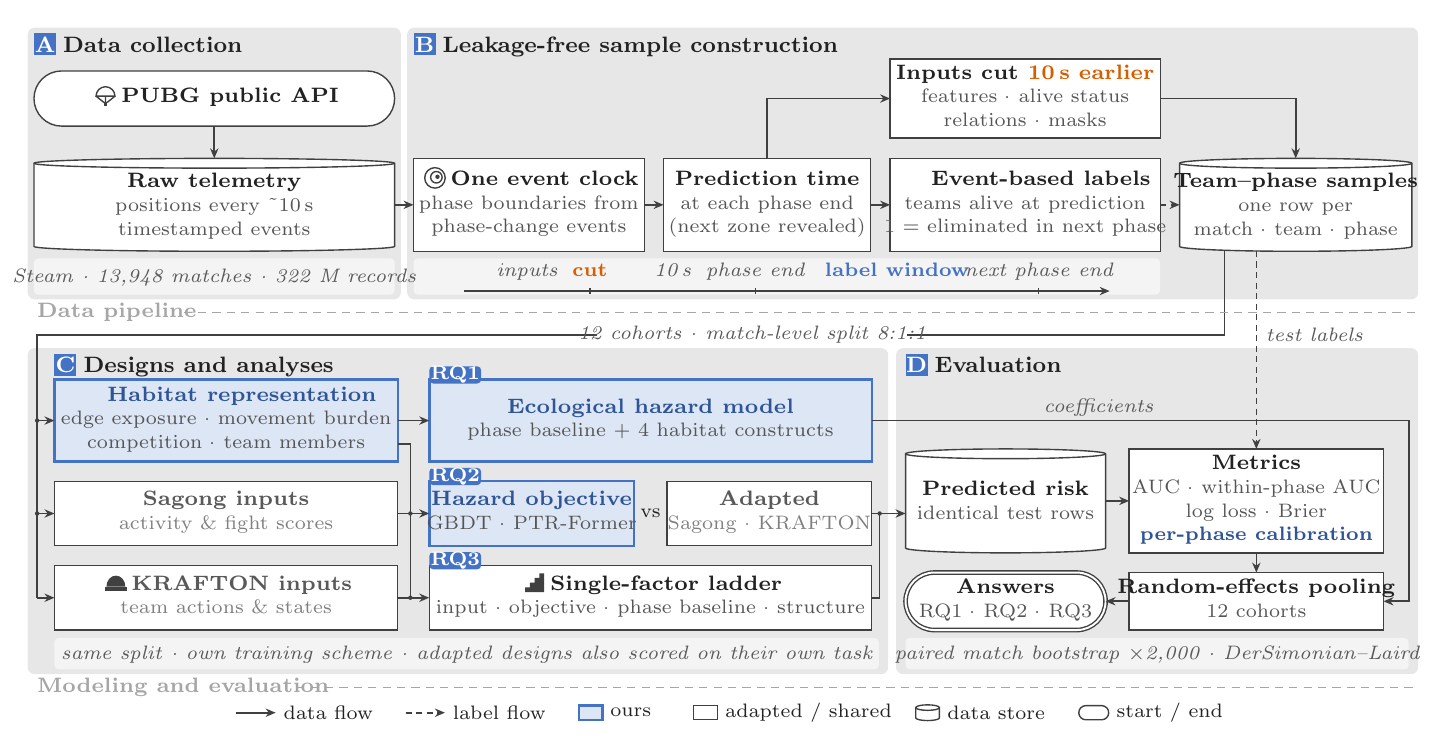
\begin{tikzpicture}
\useasboundingbox (0,0) rectangle ({17.8cm-4pt},8.83);
% ============================ PANELS & STRIPS ============================
% ---- panel A: Data collection
\fill[panel] (0,5.38) rectangle (4.74,8.83);
\fill[blueC] (0.08,8.48) rectangle (0.36,8.76);
% ---- panel B: Leakage-free sample construction
\fill[panel] (4.82,5.38) rectangle (17.659,8.83);
\fill[blueC] (4.9,8.48) rectangle (5.18,8.76);
% ---- panel C: Designs and analyses
\fill[panel] (0,0.62) rectangle (10.929,4.76);
\fill[blueC] (0.34,4.41) rectangle (0.62,4.69);
% ---- panel D: Evaluation
\fill[panel] (11.029,0.62) rectangle (17.659,4.76);
\fill[blueC] (11.149,4.41) rectangle (11.429,4.69);
\fill[stripF,rounded corners=1.5pt] (0.08,5.44) rectangle (4.66,5.9);
\fill[stripF,rounded corners=1.5pt] (4.9,5.44) rectangle (14.383,5.9);
\fill[stripF,rounded corners=1.5pt] (0.34,0.68) rectangle (10.809,1.08);
\fill[stripF,rounded corners=1.5pt] (11.149,0.68) rectangle (17.539,1.08);
% ============================ TOP ZONE BOXES ============================
% A1 (pill)
\draw[box,rounded corners=0.35cm] (0.08,7.58) rectangle (4.66,8.28);
% A2 (cyl)
\cyl{box}{0.08}{5.99}{4.66}{7.17}
% B1 (box)
\draw[box] (4.9,5.99) rectangle (7.83,7.17);
% B2 (box)
\draw[box] (8.076,5.99) rectangle (10.706,7.17);
% B3a (box)
\draw[box] (10.953,7.43) rectangle (14.383,8.43);
% B3b (box)
\draw[box] (10.953,5.99) rectangle (14.383,7.17);
% B4 (cyl)
\cyl{box}{14.629}{5.99}{17.579}{7.17}
% ============================ BOTTOM ZONE BOXES ============================
% C1 (ours)
\draw[ours] (0.34,3.32) rectangle (4.7,4.36);
% C2 (box)
\draw[box] (0.34,2.25) rectangle (4.7,3.07);
% C3 (box)
\draw[box] (0.34,1.18) rectangle (4.7,2);
% M1 (ours)
\draw[ours] (5.1,3.32) rectangle (10.72,4.36);
% M2L (ours)
\draw[ours] (5.1,2.25) rectangle (7.7,3.07);
% M2R (box)
\draw[box] (8.12,2.25) rectangle (10.72,3.07);
% M3 (box)
\draw[box] (5.1,1.18) rectangle (10.72,2);
% D1 (cyl)
\cyl{box}{11.149}{2.16}{13.689}{3.48}
% D2 (box)
\draw[box] (13.989,2.16) rectangle (17.219,3.48);
% D3 (box)
\draw[box] (13.989,1.18) rectangle (17.219,1.91);
% END (endpill)
\draw[box,double=white,double distance=0.7pt,rounded corners=0.365cm] (11.149,1.18) rectangle (13.689,1.91);
\fill[blueC,rounded corners=1.5pt] (5.1,4.31) rectangle (5.76,4.53);
\fill[blueC,rounded corners=1.5pt] (5.1,3.02) rectangle (5.76,3.24);
\fill[blueC,rounded corners=1.5pt] (5.1,1.95) rectangle (5.76,2.17);
% ============================ EDGES ============================
% edge A1A2: A1 -> A2
\draw[edge] (2.37,7.58) -- (2.37,7.17);
% edge A2B1: A2 -> B1
\draw[edge] (4.66,6.58) -- (4.9,6.58);
% edge B1B2: B1 -> B2
\draw[edge] (7.83,6.58) -- (8.076,6.58);
% edge B2B3a: B2 -> B3a (elbow)
\draw[edge] (9.391,7.17) -- (9.391,7.93) -- (10.953,7.93);
% edge B2B3b: B2 -> B3b
\draw[edge] (10.706,6.58) -- (10.953,6.58);
% edge B3aB4: B3a -> B4 (inputs, solid)
\draw[edge] (14.383,7.93) -- (16.104,7.93) -- (16.104,7.17);
% edge B3bB4: B3b -> B4 (labels, dashed = label flow)
\draw[dedge] (14.383,6.58) -- (14.629,6.58);
% edge RET: return line B4 -> down the left margin of C (bus), interrupted by its label "12 cohorts . match-level split 8:1:1"
\draw[lineplain] (15.2,6.003) -- (15.2,4.93) -- (11.17,4.93);
\draw[lineplain] (7.23,4.93) -- (0.12,4.93) -- (0.12,1.59);
% edge RETC1: return bus -> C1
\draw[edge] (0.12,3.84) -- (0.34,3.84);
% edge RETC2: return bus -> C2
\draw[edge] (0.12,2.66) -- (0.34,2.66);
% edge RETC3: return bus -> C3
\draw[edge] (0.12,1.59) -- (0.34,1.59);
\fill[ink] (0.12,3.84) circle (0.028);
\fill[ink] (0.12,2.66) circle (0.028);
% edge DASH: label flow B4 -> D2, straight down ("Y (test)")
\draw[dedge] (15.604,5.994) -- (15.604,3.48);
% edge C1M1: C1 -> M1 ("z")
\draw[edge] (4.7,3.84) -- (5.1,3.84);
% edge C1bus: C1 -> input bus
\draw[lineplain] (4.7,3.54) -- (4.86,3.54) -- (4.86,2.66);
% edge C2bus: C2 -> input bus
\draw[lineplain] (4.7,2.66) -- (4.86,2.66);
% edge C3bus: C3 -> input bus
\draw[lineplain] (4.7,1.59) -- (4.86,1.59);
% edge busV: vertical input bus
\draw[lineplain] (4.86,2.66) -- (4.86,1.59);
% edge busM2: bus -> M2
\draw[edge] (4.86,2.66) -- (5.1,2.66);
% edge busM3: bus -> M3
\draw[edge] (4.86,1.59) -- (5.1,1.59);
\fill[ink] (4.86,2.66) circle (0.028);
\fill[ink] (4.86,1.59) circle (0.028);
% edge M2D1: M2 -> D1 (merged arrowhead)
\draw[edge] (10.72,2.66) -- (11.149,2.66);
% edge M3D1: M3 -> joins M2 -> D1
\draw[lineplain] (10.72,1.59) -- (10.82,1.59) -- (10.82,2.66);
\fill[ink] (10.82,2.66) circle (0.028);
% edge D1D2: D1 -> D2
\draw[edge] (13.689,2.82) -- (13.989,2.82);
% edge D2D3: D2 -> D3
\draw[edge] (15.604,2.16) -- (15.604,1.91);
% edge D3END: D3 -> END
\draw[edge] (13.989,1.545) -- (13.689,1.545);
% edge M1D3: M1 -> D3 ("beta, SE"): above D1/D2, then down the right margin
\draw[edge] (10.72,3.84) -- (17.539,3.84) -- (17.539,1.545) -- (17.219,1.545);
% ============================ TIMELINE (strip B) ============================
\draw[axis] (5.541,5.485) -- (13.741,5.485);
\draw[tick] (7.141,5.45) -- (7.141,5.52);
\draw[tick] (9.241,5.45) -- (9.241,5.52);
\draw[tick] (12.841,5.45) -- (12.841,5.52);
% ============================ ZONE SEPARATORS ============================
\draw[sep] (1.98,5.21) -- (17.659,5.21);
\draw[sep] (3.41,0.45) -- (17.659,0.45);
% ============================ LEGEND ============================
\draw[edge] (2.649,0.13) -- (3.149,0.13);
\draw[dedge] (4.799,0.13) -- (5.299,0.13);
\draw[ours] (6.999,0.04) rectangle (7.299,0.22);
\draw[box] (8.459,0.04) rectangle (8.759,0.22);
\cylsmall{box}{11.279}{0.03}{11.579}{0.23}
\draw[box,rounded corners=0.09cm] (13.349,0.04) rectangle (13.729,0.22);
% ============================ TEXT (node t<ID> sits at the centre of box <ID>) ============================
\node[font=\fLetter,anchor=base,align=center,text=white] (taglA) at (0.22,8.518) {A};
\node[font=\fTitle,anchor=base west,align=left] (ttlA) at (0.45,8.518) {Data collection};
\node[font=\fLetter,anchor=base,align=center,text=white] (taglB) at (5.04,8.518) {B};
\node[font=\fTitle,anchor=base west,align=left] (ttlB) at (5.27,8.518) {Leakage-free sample construction};
\node[font=\fLetter,anchor=base,align=center,text=white] (taglC) at (0.48,4.448) {C};
\node[font=\fTitle,anchor=base west,align=left] (ttlC) at (0.71,4.448) {Designs and analyses};
\node[font=\fLetter,anchor=base,align=center,text=white] (taglD) at (11.289,4.448) {D};
\node[font=\fTitle,anchor=base west,align=left] (ttlD) at (11.519,4.448) {Evaluation};
\node[font=\fSmallI,anchor=base,align=center,text=greyT] (tstripA) at (2.37,5.595) {Steam\md{}13,948 matches\md{}322 M records};
\node[font=\fSmallI,anchor=base,align=center,text=greyT] (tstripC) at (5.575,0.805) {same split\md{}own training scheme\md{}adapted designs also scored on their own task};
\node[font=\fSmallI,anchor=base,align=center,text=greyT] (tstripD) at (14.344,0.805) {paired match bootstrap $\times$2,000\md{}DerSimonian--Laird};
\node[font=\fBox,align=center] (tA1) at (2.37,7.93) {\rule{0pt}{0.205cm}\icoParachute{}\bT{txtC}{PUBG public API}\rule[-0.095cm]{0pt}{0.095cm}};
\node[font=\fBox,align=center] (tA2) at (2.37,6.549) {\rule{0pt}{0.205cm}\bT{txtC}{Raw telemetry}\\\bD{detC}{positions every \textasciitilde10\,s}\\\bD{detC}{timestamped events}\rule[-0.095cm]{0pt}{0.095cm}};
\node[font=\fBox,align=center] (tB1) at (6.365,6.58) {\rule{0pt}{0.205cm}\icoZone{}\bT{txtC}{One event clock}\\\bD{detC}{phase boundaries from}\\\bD{detC}{phase-change events}\rule[-0.095cm]{0pt}{0.095cm}};
\node[font=\fBox,align=center] (tB2) at (9.391,6.58) {\rule{0pt}{0.205cm}\bT{txtC}{Prediction time}\\\bD{detC}{at each phase end}\\\bD{detC}{(next zone revealed)}\rule[-0.095cm]{0pt}{0.095cm}};
\node[font=\fBox,align=center] (tB3a) at (12.668,7.93) {\rule{0pt}{0.205cm}\bT{txtC}{Inputs cut \textcolor{verC}{10\,s earlier}}\\\bD{detC}{features\md{}alive status}\\\bD{detC}{relations\md{}masks}\rule[-0.095cm]{0pt}{0.095cm}};
\node[font=\fBox,align=center] (tB3b) at (12.668,6.58) {\rule{0pt}{0.205cm}\icoCrosshairs{}\bT{txtC}{Event-based labels}\\\bD{detC}{teams alive at prediction}\\\bD{detC}{1 = eliminated in next phase}\rule[-0.095cm]{0pt}{0.095cm}};
\node[font=\fBox,align=center] (tB4) at (16.104,6.549) {\rule{0pt}{0.205cm}\bT{txtC}{Team--phase samples}\\\bD{detC}{one row per}\\\bD{detC}{match\md{}team\md{}phase}\rule[-0.095cm]{0pt}{0.095cm}};
\node[font=\fBox,align=center] (tC1) at (2.52,3.84) {\rule{0pt}{0.205cm}\icoLeaf{}\bT{oursT}{Habitat representation}\\\bD{detC}{edge exposure\md{}movement burden}\\\bD{detC}{competition\md{}team members}\rule[-0.095cm]{0pt}{0.095cm}};
\node[font=\fBox,align=center] (tC2) at (2.52,2.66) {\rule{0pt}{0.205cm}\bT{greyT}{Sagong inputs}\\\bD{greyD}{activity \& fight scores}\rule[-0.095cm]{0pt}{0.095cm}};
\node[font=\fBox,align=center] (tC3) at (2.52,1.59) {\rule{0pt}{0.205cm}\icoHelmet{}\bT{greyT}{KRAFTON inputs}\\\bD{greyD}{team actions \& states}\rule[-0.095cm]{0pt}{0.095cm}};
\node[font=\fBox,align=center] (tM1) at (7.91,3.84) {\rule{0pt}{0.205cm}\bT{oursT}{Ecological hazard model}\\\bD{detC}{phase baseline + 4 habitat constructs}\rule[-0.095cm]{0pt}{0.095cm}};
\node[font=\fBox,align=center] (tM2L) at (6.4,2.66) {\rule{0pt}{0.205cm}\bT{oursT}{Hazard objective}\\\bD{detC}{GBDT\md{}PTR-Former}\rule[-0.095cm]{0pt}{0.095cm}};
\node[font=\fBox,align=center] (tM2R) at (9.42,2.66) {\rule{0pt}{0.205cm}\bT{greyT}{Adapted}\\\bD{greyD}{Sagong\md{}KRAFTON}\rule[-0.095cm]{0pt}{0.095cm}};
\node[font=\fSmall,align=center] (tvs) at (7.91,2.66) {vs};
\node[font=\fBox,align=center] (tM3) at (7.91,1.59) {\rule{0pt}{0.205cm}\icoStairs{}\bT{txtC}{Single-factor ladder}\\\bD{detC}{input\md{}objective\md{}phase baseline\md{}structure}\rule[-0.095cm]{0pt}{0.095cm}};
\node[font=\fBox,align=center] (tD1) at (12.419,2.789) {\rule{0pt}{0.205cm}\bT{txtC}{Predicted risk}\\\bD{detC}{identical test rows}\rule[-0.095cm]{0pt}{0.095cm}};
\node[font=\fBox,align=center] (tD2) at (15.604,2.82) {\rule{0pt}{0.205cm}\bT{txtC}{Metrics}\\\bD{detC}{AUC\md{}within-phase AUC}\\\bD{detC}{log loss\md{}Brier}\\\bD{detC}{{\bfseries\color{oursT}per-phase calibration}}\rule[-0.095cm]{0pt}{0.095cm}};
\node[font=\fBox,align=center] (tD3) at (15.604,1.545) {\rule{0pt}{0.205cm}\bT{txtC}{Random-effects pooling}\\\bD{detC}{12 cohorts}\rule[-0.095cm]{0pt}{0.095cm}};
\node[font=\fBox,align=center] (tEND) at (12.419,1.545) {\rule{0pt}{0.205cm}\bT{txtC}{Answers}\\\bD{detC}{RQ1\md{}RQ2\md{}RQ3}\rule[-0.095cm]{0pt}{0.095cm}};
\node[font=\fRQ,align=center,text=white] (trq1) at (5.43,4.42) {RQ1};
\node[font=\fRQ,align=center,text=white] (trq2) at (5.43,3.13) {RQ2};
\node[font=\fRQ,align=center,text=white] (trq3) at (5.43,2.06) {RQ3};
\node[font=\fSmallI,align=center,text=greyT] (tret) at (9.2,4.93) {12 cohorts\md{}match-level split 8:1:1};
\node[font=\fSmallI,anchor=west,align=left,text=greyT] (tdash) at (15.724,4.93) {test labels};
\node[font=\fSmallI,anchor=south,align=center,text=greyT] (tbeta) at (13.6,3.9) {coefficients};
\node[font=\fSmallI,anchor=base,align=center,text=greyT] (tlak) at (7.141,5.675) {\textbf{\upshape\textcolor{verC}{cut}}};
\node[font=\fSmallI,anchor=base,align=center,text=greyT] (tlbk) at (9.241,5.675) {phase end};
\node[font=\fSmallI,anchor=base,align=center,text=greyT] (tlbk1) at (12.841,5.675) {next phase end};
\node[font=\fSmallI,anchor=base,align=center,text=greyT] (tlin) at (6.341,5.675) {inputs};
\node[font=\fSmallI,anchor=base,align=center,text=greyT] (tlgd) at (8.191,5.675) {10\,s};
\node[font=\fSmallI,anchor=base,align=center,text=greyT] (tlwd) at (11.041,5.675) {\textbf{\upshape\textcolor{blueC}{label window}}};
\node[font=\fZone,anchor=west,align=left,text=zoneC] (zone1) at (0.12,5.21) {Data pipeline};
\node[font=\fZone,anchor=west,align=left,text=zoneC] (zone2) at (0.12,0.45) {Modeling and evaluation};
\node[font=\fSmall,anchor=west,align=left] (tlg0) at (3.249,0.13) {data flow};
\node[font=\fSmall,anchor=west,align=left] (tlg1) at (5.399,0.13) {label flow};
\node[font=\fSmall,anchor=west,align=left] (tlg2) at (7.399,0.13) {ours};
\node[font=\fSmall,anchor=west,align=left] (tlg3) at (8.859,0.13) {adapted / shared};
\node[font=\fSmall,anchor=west,align=left] (tlg4) at (11.679,0.13) {data store};
\node[font=\fSmall,anchor=west,align=left] (tlg5) at (13.829,0.13) {start / end};
\end{tikzpicture}
\end{document}
